\documentclass{standalone}

\usepackage{tikz}
\usetikzlibrary{3d,decorations.pathmorphing,math}
\tikzset{MyPersp/.style={
scale=2,
x={(-0.2cm,-0.4cm)},
y={(   1cm,   0cm)},
z={(   0cm,   1cm)}}}

\begin{document}

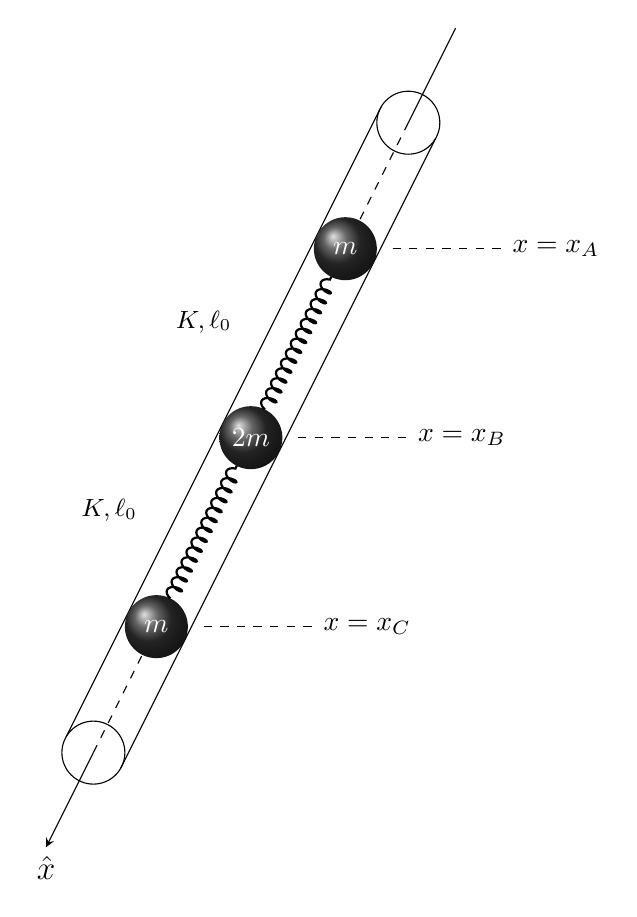
\begin{tikzpicture}[MyPersp]

\tikzmath{\xnorm = 0.447;
			 \ax =    -3;
			 \bx =     0;
			 \cx =     3;}

\begin{scope}[canvas is yz plane at x=-5]
\draw(0,0)circle(0.2);
\end{scope}

\begin{scope}[canvas is yz plane at x=5]
\draw(0,0)circle(0.2);
\end{scope}

\draw(5, {sin(60)*0.2},-{cos(60)*0.2})--(-5, {sin(60)*0.2},-{cos(60)*0.2});
\draw(5,-{sin(60)*0.2}, {cos(60)*0.2})--(-5,-{sin(60)*0.2}, {cos(60)*0.2});

\shade[ball color=black!80, x={(1cm,0cm)},y={(0cm,1cm)}](-\ax*0.2,-\ax*0.4)circle(0.2)node{\color{white}$m$};
\shade[ball color=black!80, x={(1cm,0cm)},y={(0cm,1cm)}](-\bx*0.2,-\bx*0.4)circle(0.2)node{\color{white}$2m$};
\shade[ball color=black!80, x={(1cm,0cm)},y={(0cm,1cm)}](-\cx*0.2,-\cx*0.4)circle(0.2)node{\color{white}$m$};

\draw[thick,decorate,decoration={coil,segment length=4pt}](\bx-\xnorm,0,0)--node[xshift=-1.2cm,above]{\small $K,\ell_0$}(\xnorm+\ax,0,0);
\draw[thick,decorate,decoration={coil,segment length=4pt}](\cx-\xnorm,0,0)--node[xshift=-1.2cm,above]{\small $K,\ell_0$}(\bx+\xnorm,0,0);

\draw[-stealth](5,0,0)--(6.5,0,0)node[below]{\large $\hat{x}$};
\draw[dashed]( 5,0,0)--(\cx+\xnorm,0,0);
\draw[dashed](-5,0,0)--(\ax-\xnorm,0,0);
\draw(-5,0,0)--(-6.5,0,0);

\begin{scope}[canvas is xy plane at z=0]
\draw[dashed](-3,0.3)--(-3,1)node[anchor=west]{$x=x_A$};
\draw[dashed](0 ,0.3)--( 0,1)node[anchor=west]{$x=x_B$};
\draw[dashed](3 ,0.3)--( 3,1)node[anchor=west]{$x=x_C$};
\end{scope}

\end{tikzpicture}

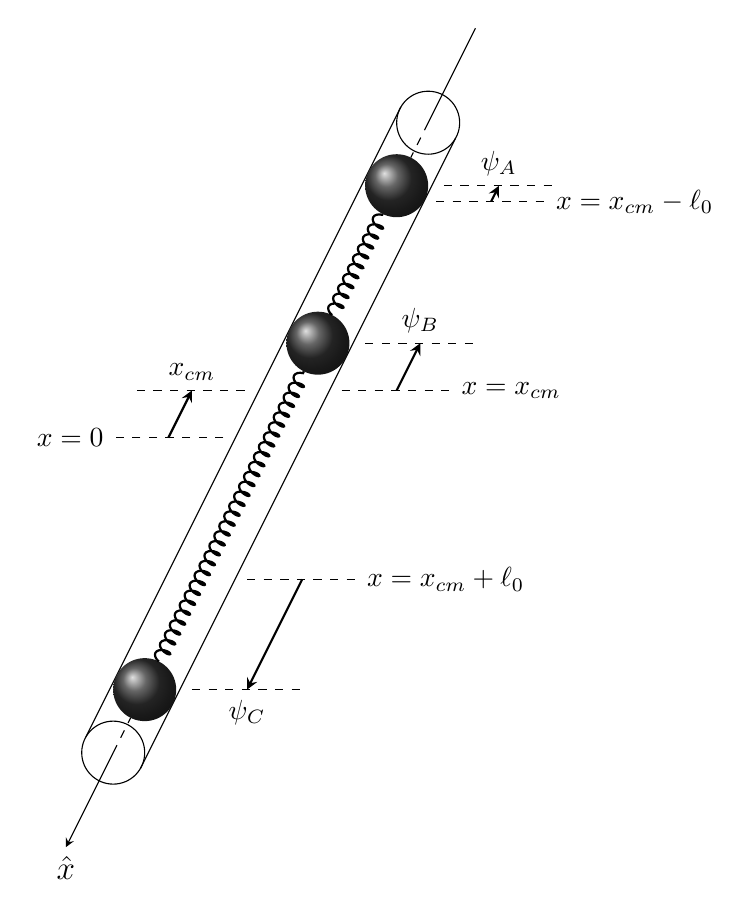
\begin{tikzpicture}[MyPersp]

\tikzmath{\xnorm  =                     0.447;
			  \ax =                        -4;
			  \bx =                      -1.5;
			  \cx =                         4;
			 \cmx = 0.25*\ax+0.5*\bx+0.25*\cx;}
			 
\begin{scope}[canvas is yz plane at x=-5]
\draw(0,0)circle(0.2);
\end{scope}

\begin{scope}[canvas is yz plane at x=5]
\draw(0,0)circle(0.2);
\end{scope}

\draw(5, {sin(60)*0.2},-{cos(60)*0.2})--(-5, {sin(60)*0.2},-{cos(60)*0.2});
\draw(5,-{sin(60)*0.2}, {cos(60)*0.2})--(-5,-{sin(60)*0.2}, {cos(60)*0.2});

\shade[ball color=black!80, x={(1cm,0cm)},y={(0cm,1cm)}](-\ax*0.2,-\ax*0.4)circle(0.2);
\shade[ball color=black!80, x={(1cm,0cm)},y={(0cm,1cm)}](-\bx*0.2,-\bx*0.4)circle(0.2);
\shade[ball color=black!80, x={(1cm,0cm)},y={(0cm,1cm)}](-\cx*0.2,-\cx*0.4)circle(0.2);

\draw[thick,decorate,decoration={coil,segment length=4pt}](\bx-\xnorm,0,0)--(\xnorm+\ax,0,0);
\draw[thick,decorate,decoration={coil,segment length=4pt}](\cx-\xnorm,0,0)--(\bx+\xnorm,0,0);

\draw[-stealth](5,0,0)--(6.5,0,0)node[below]{\large $\hat{x}$};
\draw[dashed]( 5,0,0)--(\cx+\xnorm,0,0);
\draw[dashed](-5,0,0)--(\ax-\xnorm,0,0);
\draw(-5,0,0)--(-6.5,0,0);

\begin{scope}[canvas is xy plane at z=0]
\draw[dashed](0,-0.3)--(0,-1)node[anchor=east]{$x=0$};
\draw[dashed](\cmx,-1)--(\cmx,-0.3);
\draw[-stealth,thick](0,-0.65)--(\cmx,-0.65)node[anchor=south]{$x_{cm}$};
\draw[dashed](\cmx-3,0.3)--(\cmx-3,1)node[anchor=west]{$x=x_{cm}-\ell_0$};
\draw[dashed](\cmx  ,0.3)--(\cmx  ,1)node[anchor=west]{$x=x_{cm}$};
\draw[dashed](\cmx+3,0.3)--(\cmx+3,1)node[anchor=west]{$x=x_{cm}+\ell_0$};
\foreach \i in {\ax,\bx,\cx}\draw[dashed](\i,0.3)--(\i,1);
\draw[-stealth,thick](\cmx-3,0.65)--(\ax,0.65)node[anchor=south]{$\psi_{A}$};
\draw[-stealth,thick](\cmx,0.65)--(\bx,0.65)node[anchor=south]{$\psi_{B}$};
\draw[-stealth,thick](\cmx+3,0.65)--(\cx,0.65)node[anchor=north]{$\psi_{C}$};
\end{scope}

\end{tikzpicture}

\end{document}